\chapter{Implementacija i evaluacija}
\label{chp:Implementation}

U ovom poglavlju će biti opisana implementacija pratećeg projekta nazvanog \emph{Language Invariant Code Comparer} (skr. \emph{LICC}), pisanog u programskom jeziku C\# 8.0, koristeći \emph{.NET Core 3.1} radni okvir. Lekseri i parseri za ulazne gramatike su takođe generisani u programskom jeziku C\#. C\# je izabran zbog lakoće implementacije velikih projekata i velike podrške paketa koji se mogu preuzeti, od kojih su korišćeni \emph{ANTLR Runtime} paket koji daje potrebne biblioteke za rad sa ANTLR generisanim parserima i \emph{Math.NET Symbolics} paket za rad sa simboličkim vrednostima. Rezultat je konzolna aplikacija koja može da generiše, serijalizuje ili prikaže opšti AST za dati izvorni k\^od, ali i da poredi takav AST sa drugim. Čitav projekat je dostupan u potpunosti na servisu GitHub na adresi \url{https://github.com/ivan-ristovic/LICC}.

Jedan od glavnih ciljeva aplikacije je modularnost i jednostavna proširivost. U tom duhu se, pored implementacije klasa potrebnih za predstavljanje opšte AST apstrakcije, pruža i interfejs za kreiranje adaptera koji će od proizvoljnog stabla parsiranja kreirati opšti AST. Kao primer, adapteri su kreirani za programske jezike C i Lua, a za primer potpune slobode u izboru gramatike je kreirana gramatika za pseudo-jezik i njen adapter, što dozvoljava poređenje koda sa specifikacijom datom u obliku pseudo-koda. Čitav projekat se sastoji od više komponenti, organizovanih po prostorima imena, od kojih su značajnije:
\begin{description}
    \item \texttt{LICC} --- Glavni program (korisnički interfejs) koji omogućava generisanje, prikaz, serijalizaciju i poređenje AST.
    \item \texttt{LICC.AST} ---Biblioteka klasa za rad sa opštom AST apstrakcijom.
    \item \texttt{LICC.Core} --- Upoređivač opštih AST --- konzolni izlaz.
    \item \texttt{LICC.Visualizer} --- Komponenta za vizualizaciju --- grafički prikaz AST.
    \item \texttt{LICC.Tests} --- Prateći testovi jedinica koda i integracioni testovi.
\end{description}

Arhitektura data putem UML dijagrama komponenti se može videti na slici \ref{fig:ImplementationComponents}. Osim implementacije same aplikacije, svaki funkcionalni deo projekta prate i testovi jedinica koda, koji su povezani sa \emph{GitHub Actions} podrškom za neprekidnu integraciju (engl. \emph{continuous integration}, skraćeno \emph{CI}). CI omogućava prevođenje izvornog koda nakon svake izmene kao i izvršavanje akcija nakon prevođenja kao što su testiranje ili generisanje predmeta za upotrebu (engl. \emph{artifacts}) koji predstavljaju rezultat procesa prevođenja i mogu se direktno isporučiti.

\begin{figure}[h!]
\centering
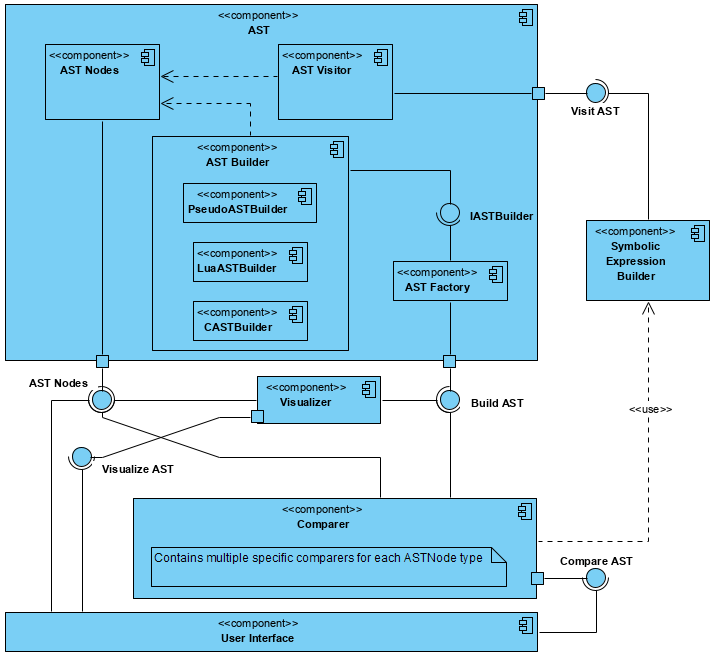
\includegraphics[scale=0.8]{images/uml/ComponentDiagram.png}
\caption{UML dijagram komponenti implementacije.}
\label{fig:ImplementationComponents}
\end{figure}


\section{Generisanje parsera uz pomoć ANTLR4}
\label{sec:ANTLRParserCreation}

U ovom odeljku će biti opisan proces generisanja leksera parsera za programske jezike C i Lua korišćenjem alata ANTLR4. Ovi programski jezici već imaju definisane ANTLR4 gramatike, tako da će se  krenuti od procesa kreiranja gramatike za programski jezik, a zatim preći na korišćenje alata ANTLR4. Nakon generisanja parsera, biće opisan i interfejs za obilazak stabla parsiranja koje generiše parser, i taj interfejs će se koristiti u procesu kreiranja opšteg AST ali i kao inspiracija za kreiranje interfejsa za obilazak opšteg AST. 


\subsection{Preduslovi za pokretanje ANTLR4}
\label{subsec:ANTLRInstallation}

Kako bi se ANTLR4 koristio, potrebno je instalirati ANTLR4 i imati \emph{Java Runtime Environment} (skr. \emph{JRE}) instaliran na sistemu i dostupan globalno pokretanjem putem komande \texttt{java}. Instalacija se sastoji od preuzimanja najnovijeg \emph{.jar} fajla\footnote{Takođe je moguće prevesti izvorni k\^od dostupan na servisu GitHub \url{https://github.com/antlr/antlr4}}, sa zvanične stranice \cite{ANTLR} ili recimo korišćenjem \emph{curl} alata\footnote{\url{https://curl.haxx.se/}}: 
\begin{lstlisting}[language={}]
$ curl -O http://www.antlr.org/download/antlr-4-complete.jar
\end{lstlisting}

Na UNIX sistemima moguće je kreirati alias \texttt{antlr4} ili \emph{shell} skript unutar direktorijuma \texttt{/usr/local/bin} sa imenom \texttt{antlr4} koji će pokrenuti \emph{.jar} fajl na sledeći način (pretpostavljajući da se \emph{.jar} fajl nalazi u direktorijumu \texttt{/usr/local/lib}):
\begin{lstlisting}[language={}]
#!/bin/sh
java -cp "/usr/local/lib/antlr4-complete.jar:$CLASSPATH" org.antlr.v4.Tool $*
\end{lstlisting}

Na Windows sistemima moguće je kreirati \emph{batch} skript sa imenom \texttt{antlr4.bat} koji će pokrenuti ANTLR4, na sledeći način (pretpostavljajući da se \emph{.jar} fajl nalazi u direktorijumu \texttt{C:\textbackslash{}lib}):
\begin{lstlisting}[language={}]
java -cp C:\lib\antlr-4-complete.jar;%CLASSPATH% org.antlr.v4.Tool %*
\end{lstlisting}

Ukoliko su aliasi ili skript fajlovi imenovani kao iznad, moguće je iz komandne linije pojednostavljeno pokretati ANTLR4:  
\begin{lstlisting}[language={}]
$ antlr4
ANTLR Parser Generator Version 4.0
-o ___    specify output directory where all output is generated
-lib ___  specify location of .tokens files
...
\end{lstlisting}

Dodatno, za Unix sisteme\footnote{Za Windows operativni sistem je moguće kreirati \emph{batch} skript po opisu na \url{https://github.com/antlr/antlr4/blob/master/doc/getting-started.md}.}, moguće je kreirati dodatni alias \texttt{grun} (ili alternativno, kreirati \texttt{shell script}) za biblioteku \texttt{TestRig}. Biblioteka \texttt{TestRig} se može koristiti za brzo testiranje parsera --- moguće je pokrenuti parser od bilo kog pravila i dobiti izlaz parsera u raznim formatima. \texttt{TestRig} dolazi uz ANTLR4 \texttt{.jar} fajl i moguće je napraviti prečicu za brzo pokretanje (nalik na ANTLR4 alias):
\begin{lstlisting}[language={}]
$ alias grun='java -cp "/usr/local/lib/antlr-4-complete.jar:$CLASSPATH" org.antlr.v4.gui.TestRig'
\end{lstlisting}


\subsection{Generisanje parsera koristeći ANTLR4}
\label{subsec:ANTLRParserGeneration}

U ovom odeljku će biti opisan proces kreiranja interfejsa za parsiranje programa pisanih u imperativnom, strogo tipiziranom pseudo-programskom jeziku (u nastavku \emph{pseudo-jezik}), sličnom pseudokodu. Dobijeni interfejs za obilazak stabla parsiranja može da se koristi u opšte svrhe, a za potrebe ovog rada će se koristiti za generisanje apstraktnog sintaksičkog stabla za izvorni k\^od pisan u pseudo-jeziku. Najpre će biti definisana gramatika pseudo-jezika prateći ANTLR4 pravila za definisanje gramatika. Tek nakon kompletnog opisa gramatike biće iskorišćen ANTLR4 kako bi se generisao parser za pseudo-jezik. Kao i za svaki drugi imperativni jezik, treba podržati neke osnovne koncepte: \emph{identifikatore}, \emph{izraze}, \emph{naredbe} i slično.

Identifikatori su niske karaktera koje predstavljaju oznaku koja odgovara određenoj memorijskoj adresi. Identifikatori se koriste umesto sirovih vrednosti adresa kako bi k\^od bio čitljiviji i lakši za pisanje --- na nivou asemblera se većinom koriste adrese ili automatski generisane oznake. Na slici \ref{fig:PseudoDef4} se može videti definicija identifikatora. Identifikator se sastoji od slova, cifara i simbola \texttt{\_}, s tim što ne sme početi cifrom. Ovo je konvencija koju prati dosta jezika, uključujući programski jezik C. Primetimo da je identifikator nešto što bi lekser trebalo da prepozna tokom tokenizacije. Međutim, kada definišemo gramatiku od koje će ANTLR4 praviti lekser i parser, možemo i tokene definisati na isti način kao i gramatička pravila dajući regularni izraz za njihovo poklapanje. Listovi stabla parsiranja su uvek tokeni, drugim rečima se nazivaju i \emph{terminalni simboli}. Tokeni se, osim u listovima, mogu naći bilo gde u stablu parsiranja. ANTLR4 dozvoljava jednostavne definicije pravila u kojima figuriše promenljiv broj drugih pravila, pri čemu se koriste simboli kao u regularnim izrazima\footnote{U regularnim izrazima, simbol \texttt{a?} označava opciono pojavljivanje simbola \texttt{a}, simbol \texttt{a+} označava jedno ili više pojavljivanja simbola \texttt{a}, a simbol \texttt{a*} označava proizvoljan broj pojavljivanja simbola \texttt{a} --- kombinacija simbola \texttt{?} i \texttt{+}.}, što je iskorišćeno za definiciju pravila za definisanje identifikatora.

\begin{figure}[h!]
\begin{lstlisting}[language={}]
NAME
    : [a-zA-Z_][a-zA-Z_0-9]*
    ;
\end{lstlisting}
\caption{Definicija identifikatora za pseudo-jezik.}
\label{fig:PseudoDef4}
\end{figure}

Po ugledu na imperativni stil, pseudo-jezik treba da bude strogo tipiziran. Stoga je potreban  koncept tipa podataka (videti definiciju deklaracije), čija je definicija data na slici \ref{fig:PseudoDef5}. Tip može biti \emph{primitivan} (drugim rečima \emph{prost}) ili \emph{složen}. Primitivni tipovi su podržani u samoj sintaksi jezika --- u našem slučaju brojevni tipovi i niske. Brojevi mogu biti celi (\texttt{integer}) ili realni (\texttt{real}). U složene tipove spadaju korisnički definisani tipovi (sa imenom \texttt{NAME}, u četvrtoj alternativi pravila \texttt{typename} sa slike \ref{fig:PseudoDef5}) i kolekcije. Od kolekcija su podržani nizovi, liste i skupovi. Prilikom definicije kolekcije mora se navesti tip elemenata kolekcije i taj tip mora biti uniforman --- isti za sve elemente kolekcije. Specijalne reči kao što su \texttt{integer} ili \texttt{array} će biti rezervisane reči našeg pseudo-jezika, tzv.~\emph{ključne reči}. Ključne reči se u pravilima navode između apostrofa.

\begin{figure}[h!]
\begin{lstlisting}[language={}]
type 
    : typename 'array'?
    | typename 'list'?
    | typename 'set'?
    ;
typename 
    : 'integer' 
    | 'real' 
    | 'string' 
    | NAME 
    ;
\end{lstlisting}
\caption{Definicija tipa podataka za pseudo-jezik.}
\label{fig:PseudoDef5}
\end{figure}

Izrazi, iako definisani rekurzivno, se mogu posmatrati kao kombinacija promenljivih, operatora i poziva funkcija sa odlikom da se mogu \emph{evaluirati}, tj. moguće je izračunati njihovu vrednost. Iz definicije pravila \texttt{exp} sa slike \ref{fig:PseudoDef6}, mogu se uočiti tipovi izraza, pri čemu nije vođeno računa o matematičkom prioritetu operatora, radi jednostavnosti. Izraz može biti \emph{literal}, koji predstavlja konstantu, bilo brojevnu, logičku ili nisku karaktera. Promenljive, definisane pravilom \texttt{var} su takođe izrazi, jer se trenutna vrednost promenljive posmatra kao vrednost izraza. Primetimo da promenljiva može biti kolekcijskog tipa, u kom slučaju se navodi redni broj elementa nakon identifikatora promenljive --- taj redni broj može biti rezultat evaluacije drugog izraza, ali ne bilo kakvog, stoga se u pravilu \texttt{iexp} definiše šta sve može biti korišćeno da se indeksira element kolekcije. Izrazima se može dati prioritet pomoću zagrada, što se vidi u trećoj alternativi pravila \texttt{exp}. U naredne tri alternative su opisani tipovi izraza: aritmetički, relacioni i logički. Aritmetički izrazi su vezani aritmetičkim operatorima definisanim preko pravila \texttt{aop}, slično važi i za ostala dva tipa. Svi tipovi izraza navedeni iznad su vezani binarnim operatorima, što znači da oni zahtevaju dva argumenta. Postoje i unarni operatori, od kojih su podržani operatori promene znake i logičke negacije, što se vidi iz pravila \texttt{uop}. Poziv funkcije je takođe validan izraz jer funkcije imaju povratne vrednosti i on je označen imenom \texttt{cexp} (skraćeno od \emph{function call expression})\footnote{Funkcije mogu vratiti vrednosti pa se stoga njihovi pozivi mogu naći u izrazima --- dakle poziv funkcije je validan izraz (stoga \texttt{expression} u imenu \texttt{function call expression}). Naravno, ta vrednost se može ignorisati ili pak sama funkcija može biti takva da nema povratnu vrednost već je samo neophodno izvršiti je zbog sporednih efekata.}.

\begin{figure}[h!]
\begin{lstlisting}[language={}]
exp
    : literal 
    | var
    | '(' exp ')'
    | exp aop exp
    | exp rop exp
    | exp lop exp
    | uop exp
    | cexp
    ;
var 
    : NAME ('[' iexp ']')?
    ;
iexp 
    : literal
    | var
    | aexp
    ;
cexp
    : 'call' NAME '(' explist? ')'
    ;
explist
    : exp (',' exp)*
    ;
aop : '+' | '-' | '*' | '/' | 'div' | 'mod' ;
rop : '>' | '>=' | '<' | '<=' | '==' | '=/=' ;
lop : 'and' | 'or' ;
uop : '-' | 'not' ;
\end{lstlisting}
\caption{Definicija izraza za pseudo-jezik.}
\label{fig:PseudoDef6}
\end{figure}

Definicija literala je prikazana na slici \ref{fig:PseudoDef7}. Literali mogu bili istinitosne konstante \texttt{True} i \texttt{False}, brojevne konstante ili niske karaktera. Brojevne konstante mogu bili celobrojni ili realni dekadni brojevi. Realne konstante je moguće definisati u fiksnom ili pokretnom zarezu. Niske se mogu definisati između navodnika ili apostrofa. Pritom, kao i u modernim programskim jezicima, moguće je navesti sekvence koje predstavljaju specijalne karaktere kao što su novi red, tabulator itd. Oznaka \texttt{fragment} označava optimizaciju, naime nije potrebno da postoji, na primer, pravilo \texttt{Digit}, već samo dajemo simbol za regularni izraz koji će se koristiti u više drugih pravila i poklapati jednu dekadnu cifru.

\begin{figure}[h!]
\begin{lstlisting}[language={}]
literal : 'True' | 'False' | INT | FLOAT | STRING ;
STRING : '"' ( EscapeSequence | ~('\\'|'"') )* '"'  ;
INT : Digit+ ;
FLOAT
    : Digit+ '.' Digit* ExponentPart?
    | '.' Digit+ ExponentPart?
    | Digit+ ExponentPart
    ;

fragment
ExponentPart : [eE] [+-]? Digit+ ;
fragment
Digit : [0-9] ;
fragment
EscapeSequence : '\\' [abfnrtvz"'\\] | '\\' '\r'? '\n' ;
\end{lstlisting}
\caption{Definicija konstanti za pseudo-jezik.}
\label{fig:PseudoDef7}
\end{figure}

Sledeći korak je definisanje naredbi pseudo-jezika --- samostalnih izvršivih jedinica koda. Slično kao i u drugim programskim jezicima, potrebno je podržati koncept deklaracije promenljive, dodele vrednosti izraza promenljivoj, naredbe kontrole toka --- grananje i petlje. U nekim slučajevima će biti potrebno definisanje kompleksnih naredbi koje se sastoje od više drugih naredbi --- blokovi naredbi. Kako bismo označili da su naredbe deo bloka naredbi, koristićemo ključne reči \texttt{begin} i \texttt{end}, osim ukoliko je reč o samo jednoj naredbi. Na slici \ref{fig:PseudoDef2} je definisano šta se sve smatra jednom naredbom (prateći redosled alternativa pravila): prazna naredbe (označena ključnom rečju \texttt{pass}), deklaracija, dodela, poziv funkcije, vraćanje vrednosti izraza (ključna vrednost \texttt{return}) iz funkcije, prekidanje izvršavanja davanjem poruke o grešci, naredba grananja, \emph{while} petlja, \emph{repeat-until} petlja i inkrementiranje/dekrementiranje vrednosti promenljive. 
    
\begin{figure}[h!]
\begin{lstlisting}[language={}]
statement
    : 'pass'
    | declaration
    | assignment
    | cexp
    | 'return' exp
    | 'error' STRING
    | 'if' exp 'then' block ('else' block)? 
    | 'while' exp 'do' block 
    | 'repeat' block 'until' exp
    | ('increment' | 'decrement') var	
    ;
\end{lstlisting}
\caption{Definicija naredbe za pseudo-jezik.}
\label{fig:PseudoDef2}
\end{figure}

Deklaracija, prikazana na slici \ref{fig:PseudoDef3}, uvodi pojavljivanje simbola sa identifikatorom \texttt{NAME} kao oznaku za promenljivu, funkciju ili proceduru --- funkciju bez povratne vrednosti. Svaka promenljiva mora biti određenog tipa, što se postiže pravilom \texttt{type}. Promenljivoj se, opciono, može pridružiti početna vrednost, drugim rečima promenljiva se može \emph{inicijalizovati} tako da joj se pridruži vrednost nekog izraza. Procedure i funkcije imaju opcione parametre, vrednosti izraza koje im se prosleđuju kasnije u pozivu kao argumenti. Lista parametara, takođe prikazana na slici \ref{fig:PseudoDef3}, se navodi kao lista proizvoljno mnogo parova \texttt{NAME : type}, što se vidi iz definicije pravila \texttt{parlist}.

\begin{figure}[h!]
\begin{lstlisting}[language={}]
declaration
    : 'declare' type NAME ('=' exp)? 
    | 'procedure' NAME '(' parlist? ')' block 
    | 'function' NAME '(' parlist? ')' 'returning' type block 
    ;
parlist
    : NAME ':' type (',' NAME ':' type)*
    ;
\end{lstlisting}
\caption{Definicija deklaracije za pseudo-jezik.}
\label{fig:PseudoDef3}
\end{figure}

Program možemo posmatrati kao niz naredbi kome je pridružen identifikator koji označava ime programa. Na slici \ref{fig:PseudoDef1} se može videti pravilo koje definiše program\footnote{Drugim rečima, jedan program u pseudo-jeziku je jedinica prevođenja, pa je zato pravilo nazvano \emph{unit}.} i blok naredbi pseudo-jezika. Pritom, \texttt{NAME} je identifikator koji predstavlja ime programa (algoritma).

\begin{figure}[h!]
\begin{lstlisting}[language={}]
unit
    : 'algorithm' NAME block EOF
    ;
block
    : 'begin' statement+ 'end'
    | statement
    ;
\end{lstlisting}
\caption{Definicija jedinice prevođenja i bloka naredbi za pseudo-jezik.}
\label{fig:PseudoDef1}
\end{figure}

Na kraju, treba definisati sve ono što lekser treba da preskoči tokom prolaska kroz izvorni k\^od. To su beline (nevidljivi karakteri kao što su razmaci, tabulatori i novi redovi) i komentari. Definicije ovih pravila se mogu videti na slici \ref{fig:PseudoDef8}. Vidimo da se u njima koristi posebna oznaka \texttt{-> skip}, koja predstavlja instrukcije lekseru da preskoči sve ono što ovo pravilo poklopi. Komentari su u stilu kao u programskom jeziku C (ali naravno, isti stil se koristi i u mnogim jezicima) i mogu biti jednolinijski ili višelinijski. Beline koje treba preskočiti su definisane u pravilu \texttt{WS}, skraćeno od \emph{whitespace}, što u prevodu sa engleskog znači \emph{beli prostor, belina}.

\begin{figure}[h!]
\begin{lstlisting}[language={}]
BlockComment
    :   '/*' .*? '*/'  -> skip
    ;
LineComment
    :   '//' ~[\r\n]*  -> skip
    ;
WS  
    : [ \t\u000C\r\n]+ -> skip
    ;
\end{lstlisting}
\caption{Definicija komentara i belina za pseudo-jezik.}
\label{fig:PseudoDef8}
\end{figure}

Ovako definisanu gramatiku možemo sačuvati u fajl sa imenom \texttt{Pseudo.g4}, potrebno je navesti ime gramatike na početku fajla, kao na slici \ref{fig:PseudoDef9}. Naredni korak je kreiranje leksera i parsera koristeći ANTLR4, pretpostavljajući da je instaliran na način opisan u \ref{subsec:ANTLRInstallation}. Pokretanjem ANTLR-a generišemo lekser i parser za gramatiku pseudo-jezika:
\begin{lstlisting}[language={}]
$ antlr4 Pseudo.g4
\end{lstlisting}

\begin{figure}[h!]
\begin{lstlisting}[language={}]
grammar Pseudo;
\end{lstlisting}
\caption{Definicija imena gramatike za pseudo-jezik.}
\label{fig:PseudoDef9}
\end{figure}

ANTLR4 će generisati lekser i parser podrazumevano napisane u programskom jeziku Java u odvojenim izvornim fajlovima kao zasebne klase. Ukoliko želimo to da promenimo, možemo koristiti opciju \texttt{-Dlanguage=...}. 

Kako bismo testirali generisani lekser i parser, možemo koristiti ANTLR4 \texttt{TestRig} da vizualno prikažemo stablo parsiranja, s tim što moramo prvo kompilirati generisane Java klase. \texttt{TestRig} pozivamo navođenjem imena gramatike (koje se poklapa sa imenom leksera i parsera) i imenom pravila od koga će parser krenuti. Opcija \texttt{-gui} pokreće vizualni prikaz stabla parsiranja prikazan na slici \ref{fig:PseudoTreeGui} (vizualni prikaz je moguće preskočiti i samo ispisati stablo u LISP formi koristeći opciju \texttt{-tree}), mada je moguće i ispisati samo tokene koristeći opciju \texttt{-tokens}. Ulaz se prosleđuje programu dok se ne naiđe na simbol \texttt{EOF}, ili alternativno se može preneti ulaz putem UNIX pipeline-a (na slici \ref{fig:PseudoTreeGui} se može videti izlaz koji se dobija korišćenjem opcije \texttt{-gui}):
\begin{lstlisting}[language={}]
$ javac *.java
$ echo "declare integer x = 5" | grun Pseudo declaration -tokens
[@0,0:6='declare',<'declare'>,1:0]
[@1,8:14='integer',<'integer'>,1:8]
[@2,16:16='x',<NAME>,1:16]
[@3,18:18='=',<'='>,1:18]
[@4,20:20='5',<INT>,1:20]
[@5,22:21='<EOF>',<EOF>,2:0]
$ echo "declare integer x = 5" | grun Pseudo declaration -tree
(declaration declare (type (typename integer)) x = (exp (literal 5)))
$ echo "declare integer x = 5" | grun Pseudo declaration -gui
\end{lstlisting}    

\begin{figure}[h!]
\centering
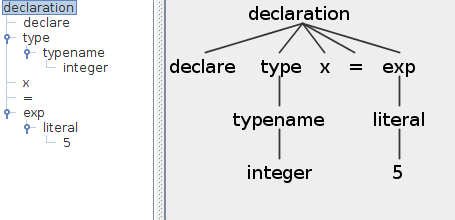
\includegraphics[scale=0.8]{images/pseudo_parse_tree.png}
\caption{Grafički prikaz stabla parsiranja koje generiše parser kreiran od strane \texttt{TestRig} biblioteke za naredbu deklaracije celobrojne promenljive u pseudo-jeziku.}
\label{fig:PseudoTreeGui}
\end{figure}


\subsection{Obilazak stabla parsiranja}
\label{subsec:ANTLRParserIntegration}

ANTLR4, osim leksera i parsera za datu gramatiku, može da kreira interfejse i bazne klase koji prate obrasce za projektovanje \emph{posetilac} (engl. \emph{visitor}) i osluškivač (engl. \emph{listener})\footnote{Osluškivač je varijanta obrasca \emph{posmatrač} (engl. \emph{observer})} opisane u \ref{sec:DesignPatterns}. Tako kreirani interfejsi i klase imaju metode za obilazak stabla parsiranja. ANTLR4 podrazumevano generiše interfejs osluškivača (slika \ref{fig:ANTLRListener}) kao i baznu klasu koja implementira generisani interfejs tako što su sve implementirane metode prazne. Stoga, ukoliko korisnik želi da definiše operaciju samo u slučaju da se prilikom obilaska stabla parsiranja naiđe na određeni tip čvora, nije potrebno implementirati ceo interfejs osluškivača već je moguće naslediti baznu klasu i predefinisati samo jedan metod. ANTLR4 može, pored osluškivača, da generiše i posetilac (slika \ref{fig:ANTLRVisitor}) ukoliko se navede odgovarajuća opcija \texttt{-visitor} prilikom pokretanja. Slično, ukoliko nije potrebno generisati osluškivač, može se koristiti opcija \texttt{-no-listener}.

\begin{figure}[h!]
\begin{lstlisting}
public interface IPseudoListener : IParseTreeListener
{
    void EnterUnit([NotNull] PseudoParser.UnitContext context);
    void ExitUnit([NotNull] PseudoParser.UnitContext context);
    void EnterBlock([NotNull] PseudoParser.BlockContext context);
    void ExitBlock([NotNull] PseudoParser.BlockContext context);
    void EnterStatement([NotNull] PseudoParser.StatementContext context);
    void ExitStatement([NotNull] PseudoParser.StatementContext context);
    
    ...
}
\end{lstlisting}
\caption{Delimični prikaz interfejsa osluškivača generisanog od strane ANTLR4 za pseudo-jezik definisan u prethodnom odeljku (C\#).}
\label{fig:ANTLRListener}
\end{figure}

Sa slike \ref{fig:ANTLRListener} se vidi da je moguće definisati metode koje će se pozivati prilikom ulaska ali i prilikom izlaska iz čvora određenog tipa prilikom obilaska stabla parsiranja. Pritom je važno kako se stablo obilazi. U slučaju ANTLR4, to je pretraga u dubinu (engl. \emph{depth-first search, DFS})\footnote{DFS je obilazak stabla takav da se obilazak duž grane stabla nastavlja sve dok je moguće ići dublje, a ako to nije moguće vratiti se unazad i obići druge grane.}, stoga će se metod \texttt{Exit} za proizvoljni čvor pozvati tek kad se obiđu sva deca tog čvora --- dakle nakon poziva njihovih \texttt{Enter} i \texttt{Exit} metoda. Pošto se DFS obično implementira putem LIFO strukture\footnote{\emph{Last In, First Out} struktura podataka je apstraktna struktura podataka sa operacijama ubacivanja i izbacivanja elemenata, pri čemu je element koji se izbacuje onaj koji je poslednji ubačen. Primer LIFO strukture je držač za CD-ove --- ne mogu se ukloniti CD-ovi ispod CD-a na vrhu (poslednji ubačen) a da se ne ukloni isti. U slučaju opisanom iznad, implementacija LIFO strukture se naziva stek (engl. \emph{stack}).}, može se reći da se \texttt{Enter} metod poziva onog trenutka kad se čvor ubaci u strukturu, a \texttt{Exit} metod onda kada se čvor ukloni iz strukture.

\begin{figure}[h!]
\begin{lstlisting}
public interface IPseudoVisitor<T> : IParseTreeVisitor<T>
{
    T VisitUnit([NotNull] PseudoParser.UnitContext context);
    T VisitBlock([NotNull] PseudoParser.BlockContext context);
    T VisitStatement([NotNull] PseudoParser.StatementContext context);
    T VisitDeclaration([NotNull] PseudoParser.DeclarationContext context);
    
    ...
}
\end{lstlisting}
\caption{Delimični prikaz interfejsa posetioca generisanog od strane ANTLR4 za pseudo-jezik definisan u prethodnom odeljku (C\#).}
\label{fig:ANTLRVisitor}
\end{figure}

Za razliku od osluškivača, posetilac je prirodnije koristiti ukoliko je potrebno izvršiti neko izračunavanje nad strukturom koja se obilazi. Interfejs posetioca (slika \ref{fig:ANTLRVisitor}) je šablonski, i metodi imaju povratnu vrednost šablonskog tipa za razliku od metoda osluškivača i, u odnosu na osluškivač, nema para metoda za svaki čvor već samo jedan metod. Dodatna razlika, ali i najveća, je ta što se metodi posetioca ne pozivaju automatski. Stoga je na programeru da nastavi obilazak i da odluči u koje čvorove želi da se spusti. Jasno je da i osluškivač i posetilac imaju svoje primene --- ukoliko je potrebno obići stablo parsiranja i dovući neke informacije može se iskoristiti osluškivač jer onda ne moramo brinuti o obilasku. S druge strane, ukoliko je potrebno izračunati neku vrednost prirodno je iskoristiti rekurziju i iskoristiti posetilac --- rekurzivni pozivi prilikom obilaska nam idu u prilog jer koristimo povratne vrednosti tih metoda da gradimo rezultat od listova ka korenu stabla parsiranja. U nastavku će se koristiti posetilac zbog kontrole obilaska ali i činjenice da se stablo parsiranja obilazi sa ciljem da se izgradi AST, koji je takođe rekurzivna struktura i gradi se inkrementalno kroz rekurziju.

Bilo da se koristi osluškivač ili posetilac, potrebno je nekako proslediti informacije o samom čvoru na koji se naišlo tokom obilaska stabla parsiranja. Te informacije se metodima osluškivača i posetioca prosleđuju putem potklasa apstrakne klase konteksta pravila \texttt{ParserRuleContext} --- u primeru iznad \texttt{UnitContext}, \texttt{BlockContext} itd. Svaki kontekst pravila po imenu odgovara pravilima definisanim u gramatici i sadrži informacije bitne za trenutni čvor u stablu parsiranja koji odgovara tipu konteksta. Takođe, u svakom kontekstu su prisutne i metode čija imena odgovaraju pravilima koja se javljaju u definiciji samog pravila koje odgovara kontekstu. Stoga za \texttt{BlockContext}, imajući u vidu definiciju sa slike \ref{fig:PseudoDef1} gde se koristi i pravilo \texttt{statement}, u okviru \texttt{BlockContext} klase biće implementiran i metod \texttt{statement()} koji vraća kontekst pravila tipa \texttt{StatementContext[]}. Metod \texttt{statement()} vraća niz jer u prvoj alternativi stoji \texttt{statement+} --- dakle možemo imati više \texttt{statement} poklapanja. Sa ovim u vidu, moguće je odrediti kako će se obilazak nastaviti (u slučaju posetioca) ili dovući informacije o delovima definicije pravila. Ukoliko pravilo ima više alternativa, metodi koje vraćaju kontekst pravila koje figuriše u alternativi koja nije korišćena za poklapanje pravila će vratiti \texttt{null}. Pošto se \texttt{statement} pravilo javlja u obe alternative pravila \texttt{block} (i nije opciono), možemo biti sigurni da povratna vrednost \texttt{statement()} metoda nikada neće biti \texttt{null}.

\section{Implementacija opšteg AST}
\label{sec:ImplementationMyAST}

Implementacija prati hijerarhije opisane u poglavlju \ref{chp:MyAST} kroz mehanizam nasleđivanja. Svaki tip čvora je implementiran kao zasebna klasa koja direktno ili tranzitivno nasleđuje apstraktnu klasu \texttt{ASTNode}. Klase koje čine apstrakciju zajedno sa njihovom hijerarhijom se može videti na slikama \ref{fig:UMLASTNode1}, \ref{fig:UMLASTNode2} i \ref{fig:UMLASTNode3}. 

\begin{figure}[h!]
\centering
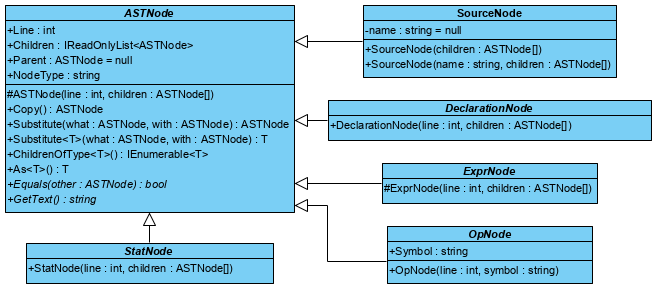
\includegraphics[scale=0.7]{images/uml/ASTNode.png}
\line(1,0){450}\\
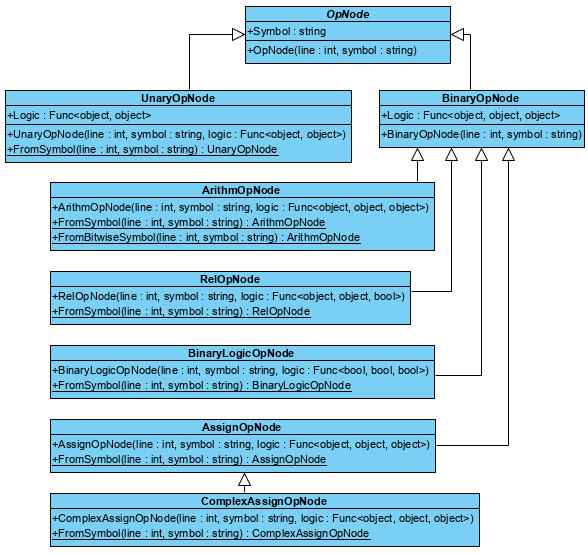
\includegraphics[scale=0.7]{images/uml/OperatorNode.png}
\caption{UML klasni dijagram opšte apstrakcije (deo 1).}
\label{fig:UMLASTNode1}
\end{figure}

\begin{figure}[h!]
\centering
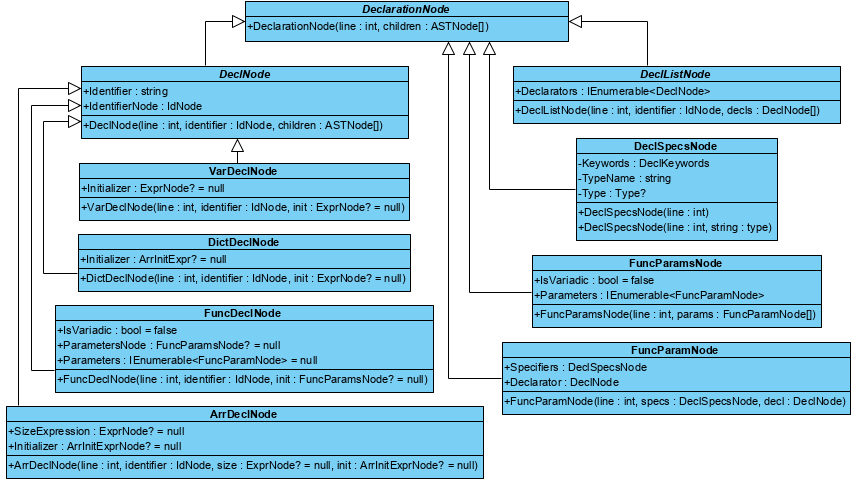
\includegraphics[scale=0.7]{images/uml/DeclarationNode.png}
\caption{UML klasni dijagram opšte apstrakcije (deo 2).}
\label{fig:UMLASTNode2}
\end{figure}

\begin{figure}[h!]
\centering
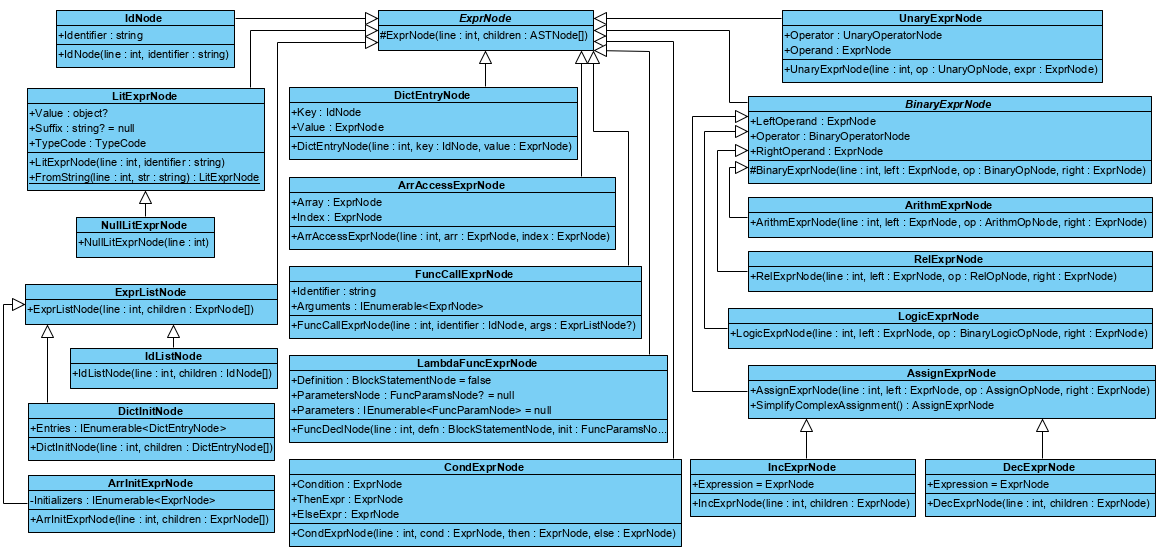
\includegraphics[scale=0.55]{images/uml/ExpressionNode.png}
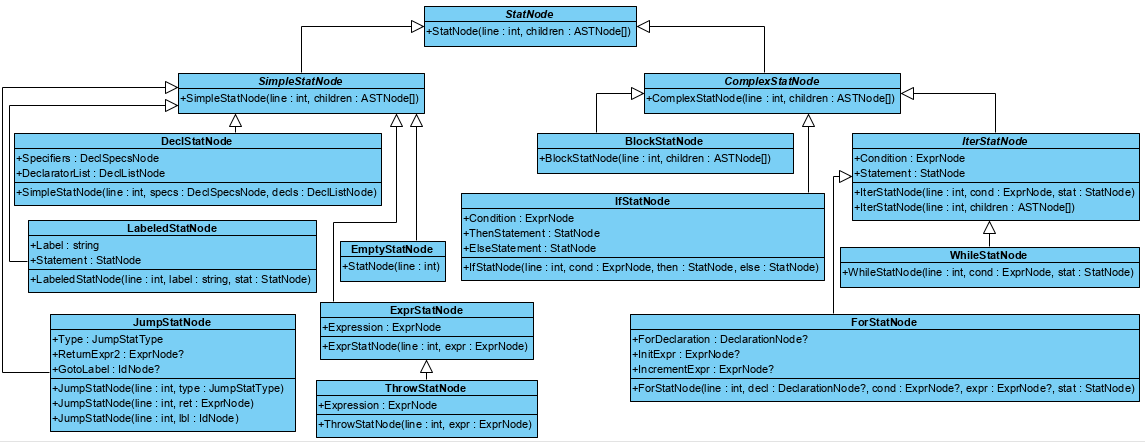
\includegraphics[scale=0.55]{images/uml/StatementNode.png}
\caption{UML klasni dijagram opšte apstrakcije (deo 3).}
\label{fig:UMLASTNode3}
\end{figure}

Jednom kreirani AST čvor je \emph{nepromenljiv}, što znači da je i ceo AST nepromenljiv --- ne mogu se dodavati ili uklanjati deca čvorovima u stablu. Međutim, moguće je klonirati AST čvorove ili vršiti zamenu određenog podstabla drugim podstablom ne menjajući original tako što se vraća izmenjena kopija originala. Svaki AST čvor se može porediti po jednakosti sa drugim AST čvorom po intuitivnoj logici poređenja pruženom kroz predefinisane operatore poređenja. Dostupne su i ekstenzije koje omogućavaju serijalizaciju stabla u JSON format.

Pored implementacije klasa koje predstavljaju AST čvorove, kreiran je i javno dostupni način za obilazak AST putem obrazca posetilac kroz apstraktnu klasu \texttt{BaseASTVisitor<TResult>}. Ova klasa ima implementirane javne virtualno predefinisani metod \texttt{TResult Visit(ASTNode node)} jednog argumenta za svaki mogući tip koji nasleđuje tip \texttt{ASTNode}. Svi ti metodi su definisani tako da se pozove metod \texttt{VisitChildren(ASTNode)} koji će posetiti svu decu trenutnog čvora. Svaki naredni rezultat poziva metoda \texttt{Visit()} za svako dete se agregira pozivanjem metoda \texttt{TResult AggregateResult(TResult curr, TResult next)} koji podrazumevano samo vraća \texttt{next}. Dodatno, moguće je predefinisati metod \texttt{bool ShouldVisitNextChild(ASTNode node, TResult curr)} koji određuje da li je potrebno prekinuti posećivanje pre nego što se posete sva deca. Ovaj metod se poziva svaki put pre nego što se poseti dete i podrazumevano vraća \texttt{true}. \texttt{BaseASTVisitor} klasa je u implementaciji korišćena za kreiranja graditelja simboličkog izraza od sintaksičkog stabla izraza kao i evaluatora takvog stabla izraza. 

Adapteri ili graditelji se koriste kao spona između stabla parsiranja za konkretni programski jezik i opšte AST apstrakcije. Uloga adaptera je da od stabla parsiranja kreiraju opšti AST. Kako bi se pružio ujednačen način za kreiranje adaptera, pružena su dva interfejsa prikazana na slici \ref{fig:ImplBuilderInterface}.

\begin{figure}[h!]
\centering
\begin{lstlisting}
public interface IAbstractASTBuilder
{
    ASTNode BuildFromSource(string code);
}

public interface IASTBuilder<TParser> : IAbstractASTBuilder where TParser : Parser
{
    TParser CreateParser(string code);
    ASTNode BuildFromSource(string code, Func<TParser, ParserRuleContext> entryProvider);
}
\end{lstlisting}
\caption{Interfejs graditelja opšteg AST od stabla parsiranja.}
\label{fig:ImplBuilderInterface}
\end{figure}

Postupak kreiranja AST za dati izvorni fajl se sastoji iz više koraka. Prvo se izvlači ekstenzija izvornog fajla. Zatim se putem refleksije pronalazi klasa koja implementira interfejs \texttt{IAbstractASTBuilder} i ima u sebi prisutan atribut \texttt{ASTBuilderAttribute(string)}\footnote{Atributi u C\#-u su deklarativni tagovi (nalik na anotacije u Java programskom jeziku) koji se koriste da se raznim elementima pridruže informacije dostupne u toku prevođenja. Ti elementi mogu biti klase, metode, osobine itd. Atributi se definišu kao klase i mogu imati polja i konstruktore s tim što vrednosti atributa moraju biti poznate za vreme prevođenja --- konstante.}
čija se niska poklapa sa ekstenzijom izvornog fajla. Naposletku se kreira instanca pronađene klase i, na osnovu toga što implementira interfejs \texttt{IAbstractASTBuilder}, poziva se metod \texttt{BuildFromSource()} za sadržaj izvornog fajla.

Dedukovani adapter implementira uvek \texttt{IASTBuilder} interfejs na osnovu tipa parsera koji je generisao ANTLR alat za gramatiku konkretnog programskog jezika. Metod \texttt{CreateParser()} instancira parser odgovarajućeg tipa. Razlog zašto ovaj proces nije uniforman je taj što se pre kreiranja parsera uvek kreira i lekser koji prvi dobija tok podataka pa se tek onda kreira parser. Dodatno, prilikom kreiranja parsera se definiše i pravilo gramatike od kojeg parser kreće (tzv. \emph{ulazno pravilo}, engl. \emph{entry rule}) koje je specifično za programski jezik. Stoga je nemoguće kreirati jedinstveni niz operacija koji će kreirati svaki parser pa se to radi prilikom implementacije adaptera. 

Predefinisani metod \texttt{BuildFromSource()} interfejsa \texttt{IASTBuilder} treba da obiđe stablo parsiranja počev od pravila koje se dobija pozivom funkcije prosleđene kao drugi argument za dati tip parsera. Ovo je generalizacija kreiranja parsera i na prvi pogled izgleda suvišno jer, pošto se parsira validan izvorni k\^od, mora se uvek krenuti od podrazumevanog ulaznog pravila za konkretni programski jezik. Međutim, ovaj način kreiranja AST je pogodan prilikom testiranja jedinica koda, jer ukoliko se npr. testira generisanje AST od izraza, nije potrebno pisati čitave funkcije sa naredbama samo da bi se testiralo generisanje apstrakcije izraza, već je moguće samo navesti izraz i instrukovati adapter da kreira parser tako da on počne od pravila koje definiše izraz.

\section{Implementacija semantičkog upoređivača}
\label{sec:ImplementationComparer}

Implementacija algoritma upoređivača opisana u poglavlju \ref{sec:ASTComparingAlgorithm} se svodi na implementaciju funkcija za poređenje za svaki tip AST čvora. Te funkcije su enkapsulirane u klase koje implementiraju interfejs za upoređivač čvorova. Te klase nisu javne, tako da se poređenje vrši kroz upoređivač koji poredi instance tipa \texttt{ASTNode}, a koji putem refleksije određuje konkretni tip čvorova i, ukoliko su tipovi isti, pronalazi konkretni upoređivač i poziva operaciju interfejsa upoređivača. Upoređivači međusobno pozivaju jedni druge, kako bi se logika poređenja uprostila --- pošto se naredbe deklaracije sastoje od specifikatora deklaracije i liste deklaratora, upoređivač naredbi deklaracije može pozivati upoređivač za specifikatore deklaracije i upoređivač za listu deklaratora. 

Upoređivač kao rezultat svog rada vraća kolekciju potencijalnih problema (upozorenja ili grešaka) koje je detektovao prilikom analize. Ovakav pristup je odabran zbog lakoće testiranja upoređivača, s obzirom da se može očekivati određena kolekcija problema za određeni izvorni k\^od. Problem se modeluje kao apstraktna klasa \texttt{BaseIssue} dok se upozorenja ili greške modeluju kroz njene konkretizacije \texttt{BaseWarning} i \texttt{BaseError}. Konkretne greške, kao što su npr. nedostatak deklaracija se mogu onda modelovati kao konkretizacije ovih klasa u zavisnosti od ozbiljnosti problema. 
\section{Vizualni prikaz stabla}
\label{sec:ImplementationVisualizer}

Osim serijalizacije AST u JSON format, kreiran je potprogram za vizualni prikaz AST-a (u daljem tekstu \emph{vizualizator}). Primeri izlaza vizualizatora se mogu videti na slikama iz poglavlja \ref{chp:MyAST} --- \ref{fig:MyASTExampleCDeclaration}, \ref{fig:MyASTExampleLuaDeclaration}, \ref{fig:MyASTExampleExpressions} i \ref{fig:MyASTExampleStatement}. Prikaz je izvršen koristeći nativni \texttt{Graphics} paket i, s obzirom da je u pitanju \emph{.NET Core 3.1} radni okvir, moguće je dobiti vizualni prikaz nezavisno od sistema.

Vizualizacija počiva na rekurzivnom algoritmu prikaza u dubinu --- za svaki čvor se prikažu potomci, rasporede jednako po širini, a onda se roditelj centrira u odnosu na ukupnu širinu koju zauzimaju deca. Ovaj pristup nije prostorno optimalan, zbog varijacija u broju dece za čvorove različitih tipova. Što se informacija za svaki čvor tiče, prikazuju se vrednosti svih atributa čvora zajedno sa njegovim tipom u zaglavlju kao i grane do njegovih potomaka.

\section{Korisnički interfejs}
\label{sec:ImplementationUI}

S obzirom da je aplikacija konzolna (osim dela komponente za vizualizaciju), korisnički interfejs se sastoji od argumenata komandne linije. Pokretanje programa bez argumenata pruža prikaz za pomoć u kome su nabrojane sve moguće opcije. Pomoć koja se pruža korisniku se može videti na slici \ref{fig:UIImpl}.

\begin{figure}[h!]
\centering
\begin{lstlisting}[language={}]
$ ./licc
ERROR(S):
No verb selected.

ast        AST generation commands
cmp        Compare source against the specification source
help       Display more information on a specific command.
version    Display version information.

$ ./licc ast
ERROR(S):
A required value not bound to option name is missing.

-v, --verbose    (Default: false) Verbose output
-t, --tree       (Default: false) Visualize AST tree
-o, --output     Output path
-c, --compact    (Default: false) Compact AST output
--help           Display this help screen.
--version        Display version information.

value pos. 0     Required. Source path

$ ./licc cmp
ERROR(S):
A required value not bound to option name is missing.

-v, --verbose    Set output to verbose messages.
--help           Display this help screen.
--version        Display version information.

value pos. 0     Required. Specification path.
value pos. 1     Required. Test source path.
\end{lstlisting}
\caption{Korisniči interfejs programa pružen kroz argumente komandne linije.}
\label{fig:UIImpl}
\end{figure}

Program zahteva da se kao prvi argument prosledi \emph{glagol} (engl. \emph{verb}) koji će odrediti operaciju koju program treba da izvrši. Od glagola zavisi broj i tip ostalih argumenata u nastavku. Mogući glagoli, sa svojim dodatnim opcijama, su:
\begin{itemize}
    \item \texttt{ast [-v -c -t] source-path [-o output-path]} \\
    Generiše opšti AST za izvorni k\^od na putanji \texttt{source-path} u JSON formatu i ispisuje isti na standardni izlaz, ili u fajl na putanji \texttt{output-path} ako je prisutna opcija \texttt{-o}. Moguće je generisati kompaktan JSON (bez poravnanja) navođenjem opcije \texttt{-c}. Vizualizacija u obliku stabla se prikazuje u novom prozoru ukoliko je prisutna opcija \texttt{-t}.
    \item \texttt{cmp [-v] specification-path test-path} \\
    Generiše opšti AST za izvorne kodove na putanjama \texttt{specification-path} i \texttt{test-path} i poredi generisana stabla. 
\end{itemize} 

Dodatno, svi glagoli podržavaju opciono detaljno logovanje operacija koje program izvršava navođenjem opcije \texttt{-v}. Takođe, navođenjem opcije \texttt{--help} nakon glagola se ispisuje uputstvo specifično za taj glagol. Verzija programa se može proveriti opcijom \texttt{--version}. Opcije \texttt{-o}, \texttt{-c}, \texttt{-t} i \texttt{-v} imaju svoje duže sinonime --- \texttt{--output}, \texttt{--compact}, \texttt{--tree} i \texttt{--verbose}, redom.


\section{Testovi}
\label{sec:ImplementationTests}

Komponentu za kreiranje AST i komponentu za poređenje AST prate testovi jedinica koda. Testovi su organizovani u zasebnom projektu na sledeći način:
\begin{itemize}
    \item \texttt{LICC.Tests.AST} --- Testovi za adaptere i posetioce, kao i testovi funkcionalnosti metoda klase \texttt{ASTNode}.
    \item \texttt{LICC.Tests.Core} --- Testovi upoređivača.
\end{itemize}

Radni okvir koji se koristi za testiranje je \texttt{NUnit}\footnote{\url{https://nunit.org/}} koji pruža tzv. \emph{model ograničenja} (engl. \emph{constraint model}) i time omogućava pisanje čitljivog koda. Pisanje testova po modelu ograničenja se sastoji od korišćenja jednog metoda za pisanje svih testova koji kao argumente prima objekat koji se testira i složeni objekat koji predstavlja ograničenje koje objekat koji se testira treba da zadovoljava. Primer testa pisanog u ovom radnom okviru uz model ograničenja u kontekstu implementacije ovog rada se može videti na slici \ref{fig:ImplTestsUnit}.

\begin{figure}[h!]
\centering
\begin{lstlisting}
protected FuncDefNode AssertFunctionSignature(
  string src, int line, string fname, 
  string returnType = "void", bool isVariadic = false, 
  AccessModifiers access = AccessModifiers.Unspecified,
  QualifierFlags qualifiers = QualifierFlags.None, 
  params (string Type, string Identifier)[] @params) 
{
  FuncDefNode f = this.GenerateAST(src).As<FuncDefNode>();
  this.AssertChildrenParentProperties(f);
  this.AssertChildrenParentProperties(f.Definition);
  Assert.That(f, Is.Not.Null);
  Assert.That(f.Line, Is.EqualTo(line));
  Assert.That(f.Declarator, Is.Not.Null);
  Assert.That(f.Declarator.Parent, Is.EqualTo(f));
  Assert.That(f.Keywords.AccessModifiers, Is.EqualTo(access));
  Assert.That(f.Keywords.QualifierFlags, Is.EqualTo(qualifiers));
  Assert.That(f.Identifier, Is.EqualTo(fname));
  Assert.That(f.ReturnTypeName, Is.EqualTo(returnType));
  Assert.That(f.IsVariadic, Is.EqualTo(isVariadic));
  if (@params?.Any() ?? false) {
    Assert.That(f.Parameters, Is.Not.Null);
    Assert.That(f.Parameters, Has.Exactly(@params.Length).Items);
    Assert.That(f.ParametersNode, Is.Not.Null);
    Assert.That(
      f.Parameters.Select(
        p => (p.Specifiers.TypeName, p.Declarator.Identifier)), 
          Is.EqualTo(@params)
      );
    }
  return f;
}

[Test]
public void ComplexDefinitionTest() 
{
  FuncDefNode f = this.AssertFunctionSignature(@"
    float f(const unsigned int x, ...) { return 3.0; }", 
    2, "f", "float", isVariadic: true, 
    @params: ("unsigned int", "x")
  );
  Assert.That(f.Definition.Children, Has.Exactly(1).Items);
}
\end{lstlisting}
\caption{Primer jediničnog testa za proveru generisanog AST čvora za datu funkciju.}
\label{fig:ImplTestsUnit}
\end{figure}

Osim testova jedinica koda, prisutni su i testovi integracije svih komponenti. Kao što je opisano u prethodnim odeljcima, rezultat rada adaptera je AST, dok je rezultat upoređivača za data dva stabla kolekcija problema. Ta dva odvojena procesa se onda mogu spojiti kako bi se testirala integracija te dve komponente --- dakle, od dva programa očekivati određenu kolekciju problema. Primer za \emph{swap} algoritam se može videti na slici \ref{fig:ImplTestsIntegration}.

\begin{figure}[h!]
\centering
\begin{lstlisting}
protected void Compare(ASTNode src, ASTNode dst, 
  MatchIssues? expectedIssues = null) 
{
  expectedIssues ??= new MatchIssues();
  var issues = new ASTNodeComparer(src, dst).AttemptMatch();
  Assert.That(issues, Is.EquivallentTo(expectedIssues));
}

[Test]
public override void DifferenceTests()
{
  this.Compare(
    this.FromPseudoSource(@"
      algorithm Swap 
      begin
        declare integer x = vx
        declare integer y = vy
        procedure swap()
        begin
          declare integer tmp = x
          x = y  
          y = tmp
        end
      end
    "),
    this.FromCSource(@"
      int x = vx, y = vy;
      void swap() { int tmp = x; y = tmp; x = y; }
    "),
    new MatchIssues()
      .AddError(new BlockEndValueMismatchError("x", 1, "vy", "vx"))
      .AddError(new BlockEndValueMismatchError("x", 3, "vy", "vx"))
  );
}
\end{lstlisting}
\caption{Primer kompletnog testa za algoritam \emph{swap}.}
\label{fig:ImplTestsIntegration}
\end{figure}

\section{Evaluacija}
\label{sec:ImplementationExample}

U ovom odeljku će biti prikazano nekoliko slučajeva upotrebe implementirane aplikacije. Prvo će biti pokazan primer generisanja opšteg AST u JSON formatu a zatim i primer poređenje dve implementacije istog algoritma u dva različita programska jezika. Algoritam koji će biti korišćen u nastavku kao primer je algoritam razmene vrednosti promenljivih implementiran kroz funkciju \texttt{swap} koja menja vrednosti dveju globalnih promenljivih. Na slici \ref{fig:ExampleSwap} se mogu videti implementacije ovog algoritma koje će biti polazne tačke za kreiranje opšteg AST i poređenja istih.

\begin{figure}[h!]
\begin{lstlisting}
int x = vx, y = vy;
void swap() { int tmp = y; y = x; x = tmp; }
\end{lstlisting}
\begin{lstlisting}
x = vx
y = vy
function swap()
	x, y = y, x
end
\end{lstlisting}
\begin{lstlisting}
algorithm Swap 
begin
    declare integer x = vx
    declare integer y = vy
    procedure swap()
    begin
        declare integer tmp 
        tmp = x
        x = y  
        y = tmp
    end
end
\end{lstlisting}
\caption{Izvorni kodovi algoritma \texttt{swap} u programskim jezicima C (gore), Lua (sredina) i u pseudojeziku (dole).}
\label{fig:ExampleSwap}
\end{figure}


\subsection{Generisanje opšteg AST}
\label{subsec:ImplementationExampleAST}

AST je moguće generisati od izvornog koda navođenjem glagola \texttt{ast}. Ukoliko su dostupni izvorni kodovi sa sadržajima kao na slici \ref{fig:ExampleSwap} u odgovarajućim datotekama, moguće je generisati opšti AST u JSON formatu zadavanjem glagola \texttt{ast} kao na slici \ref{fig:ExampleSwapAST}. U gornjem delu slike je prikazan samo deo izlaza zbog veličine generisanog JSON sadržaja, u srednjem delu slike je prikazan kompaktni JSON ispis zadat opcijom \texttt{-c}, dok je u donjem delu slike prikazan ispis zadat opcijom \texttt{-v} pri čemu je prikazan samo dao izlaza koji se generiše prilikom posećivanja stabla parsiranja i generisanja AST čvorova.

\begin{figure}[h!]
\centering
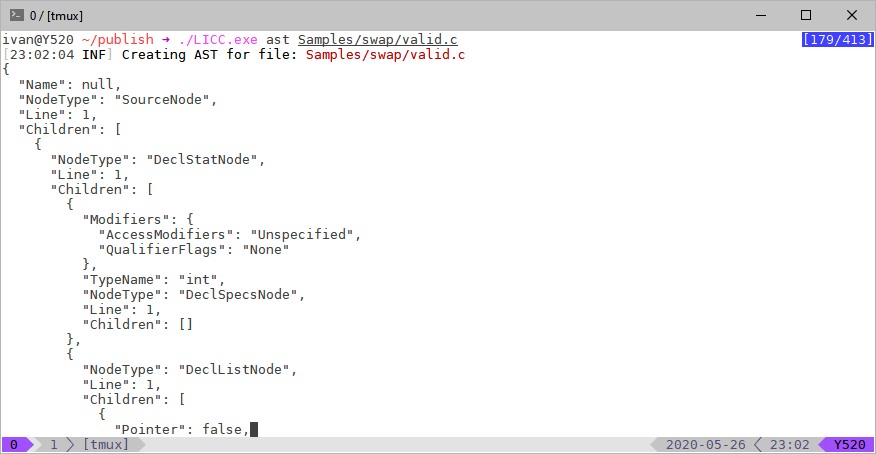
\includegraphics[scale=0.56]{images/eval/ast_c.png}
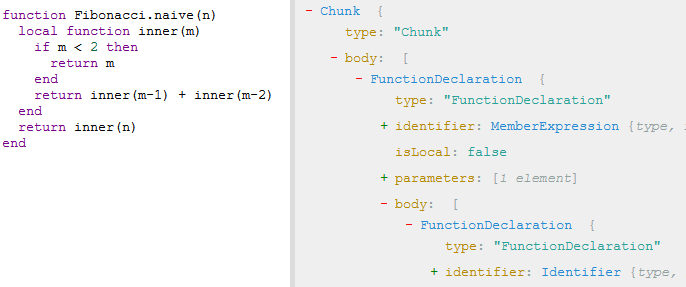
\includegraphics[scale=0.56]{images/eval/ast_lua.png}
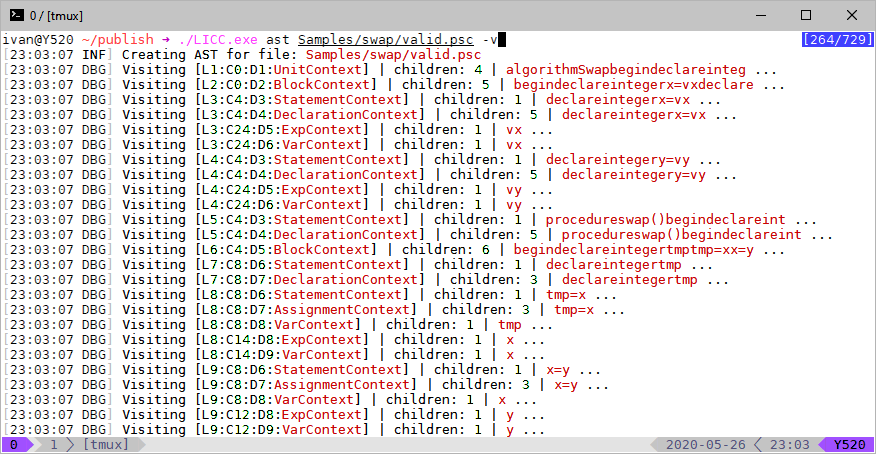
\includegraphics[scale=0.56]{images/eval/ast_psc.png}
\caption{Vizualni prikaz generisanja AST od izvornih kodova sa slike \ref{fig:ExampleSwap} redom.}
\label{fig:ExampleSwapAST}
\end{figure}


\subsection{Poređenje opštih AST}
\label{subsec:ImplementationExampleComparer}

Jedan od osnovnih slučajeva upotrebe alata LICC može biti testiranje validnosti implementacije na osnovu date specifikacije. Ukoliko kao specifikaciju za algoritam \texttt{swap} uzmemo izvorni kod u pseudo-jeziku, možemo testirati da li su implementacije u programskim jezicima C ili Lua semantički ekvivalentne specifikaciji. Izlaz rada LICC za verifikaciju implementacije algoritma \texttt{swap} u programskom jeziku Lua u odnosu na specifikaciju u pseudo-jeziku se može videti na slici \ref{fig:ExampleSwapCompareValid}. Primetimo da su prisutna upozorenja o odudaranju tipova --- Lua nije striktno tipiziran jezik, a specifikacija nalaže da su globalne promenljive celi brojevi, dok su u implementaciji one tipa \texttt{object}, što može biti potencijalni problem ali s obzirom na prirodu skript jezika nije prijavljeno kao greška.

\begin{figure}[h!]
\centering
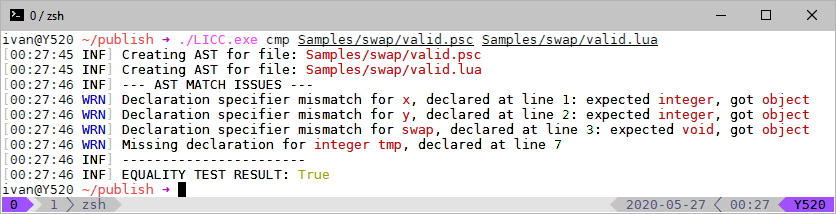
\includegraphics[scale=0.65]{images/eval/cmp_valid.png}
\caption{Semantičko poređenje implementacija sa slike \ref{fig:ExampleSwap} (Lua u odnosu na pseudo-jezik).}
\label{fig:ExampleSwapCompareValid}
\end{figure}

Ukoliko pak izvorni k\^od ne odgovara specifikaciji, LICC će dati detaljan spisak razlika, koje su često tražene greške. U nekim slučajevima je moguće da je sematnička ekvivalentnost održana iako stabla imaju značajne razlike --- LICC će prijaviti sve te razlike kao greške iako one to možda nisu. Izlaz za poređenje nevalidne implementacije algoritma \texttt{swap} sa slike \ref{fig:ExampleSwapWrong} u odnosu na specifikaciju se može videti na slici \ref{fig:ExampleSwapCompareWrong}. Vidimo da jedna od globalnih promenljivih nije pravilno zamenila vrednost, što se detektuje dvaput --- po jednom za svaki od blokova u izvornom kodu. Dodatno, prijavljena je i greška o odudaranju izraza inicijalizatora za promenljivu \texttt{tmp}.

\begin{figure}[h!]
\begin{lstlisting}
int x = vx, y = vy;
void swap() { int tmp = x; y = tmp; x = y; }
\end{lstlisting}
\caption{Nevalidna implementacija algoritma \texttt{swap} (C).}
\label{fig:ExampleSwapWrong}
\end{figure}

\begin{figure}[h!]
\centering
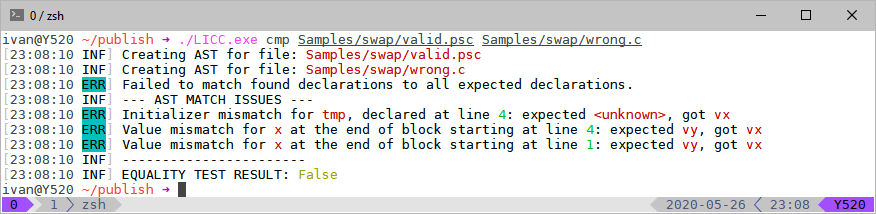
\includegraphics[scale=0.65]{images/eval/cmp_wrong.png}
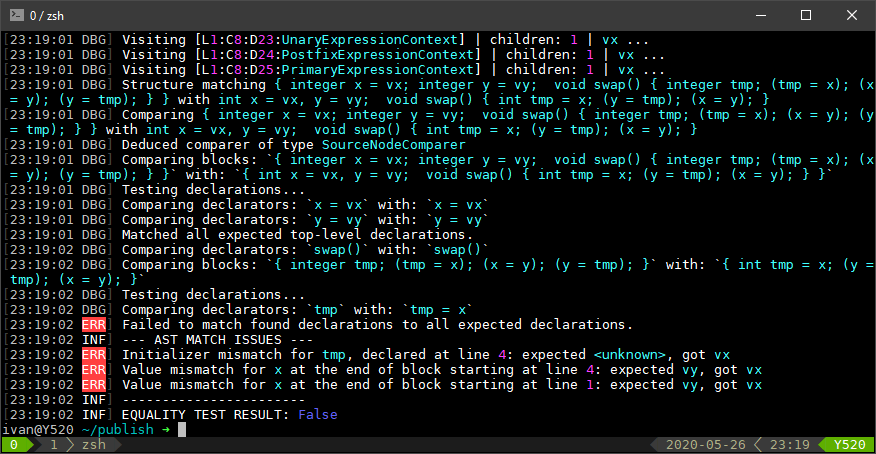
\includegraphics[scale=0.65]{images/eval/cmp_wrong_v.png}
\caption{Semantičko poređenje nevalidne implementacije sa slike \ref{fig:ExampleSwapWrong} u odnosu na specifikacije sa slike \ref{fig:ExampleSwap} -- C (gore) i pseudojezik (dole).}
\label{fig:ExampleSwapCompareWrong}
\end{figure}

Ukoliko imamo već verifikovanu implementaciju algoritma u jednom programskom jeziku, može se desiti potreba za prelaskom na novije tehnologije što uključuje i prepisivanje algoritma sa jednog programskog jezika na drugi. LICC se može iskoristiti za poređenje tih implementacija, konkretno za algoritam \texttt{swap} na slici \ref{fig:ExampleSwapCompareValidRewrite} se može videti rezultat poređenja implementacija u programskim jezicima C i Lua, pri čemu je takođe prikazan izlaz koji se dobija ukoliko se navede opcija \texttt{-v}. 

\begin{figure}[h!]
\centering
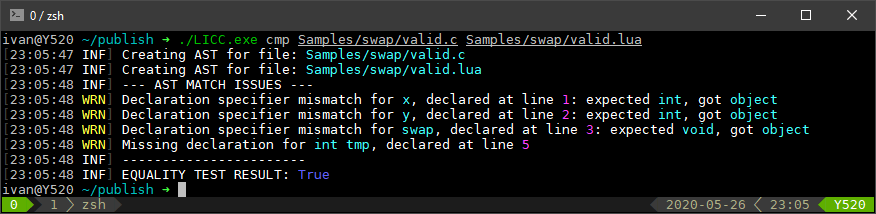
\includegraphics[scale=0.7]{images/eval/cmp_rewrite.png}
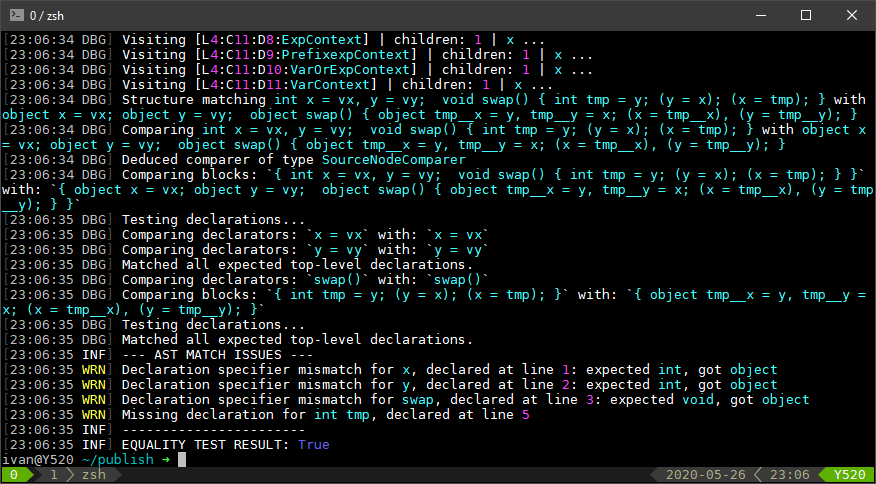
\includegraphics[scale=0.7]{images/eval/cmp_rewrite_v.png}
\caption{Semantičko poređenje implementacija sa slike \ref{fig:ExampleSwap} --- Lua u odnosu na C (gore), Lua u odnosu na pseudojezik (dole).}
\label{fig:ExampleSwapCompareValidRewrite}
\end{figure}

Još jedan slučaj upotrebe LICC može biti verifikacija međuverzija koda u procesu refaktorisanja. LICC pretpostavlja strukturnu sličnost kodova, što u procesu refaktorisanja često implicitno važi, ili barem važi u malim koracima između polazne i finalne verzije nakon refaktorisanja. Ukoliko refaktorišemo implementaciju algoritma \texttt{swap} u programskom jeziku C i dobijemo izvorni kod sa slike \ref{fig:ExampleSwapRefactor}, možemo uporediti tu implementaciju sa već verifikovanom implementacijom u programskom jeziku C. Rezultat rada upoređivača se može videti na slici \ref{fig:ExampleSwapCompareRefactor} --- primećujemo da je jedino detektovano da nedostaje promenljiva \texttt{tmp}, vrednosti globalnih promenljivih su iste u odnosu na specifikaciju na kraju svakog od blokova.

\begin{figure}[h!]
\begin{lstlisting}
int x = vx, y = vy;
void swap() { x = x + y; y = x - y; x = x - y; }
\end{lstlisting}
\caption{Refaktorisani algoritam \texttt{swap} (C).}
\label{fig:ExampleSwapRefactor}
\end{figure}

\begin{figure}[h!]
\centering
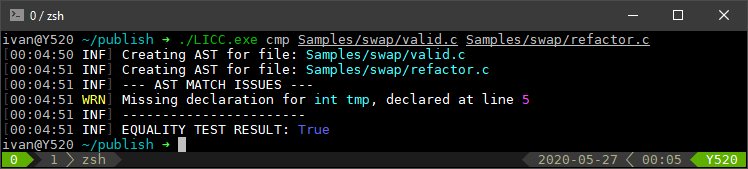
\includegraphics[scale=0.8]{images/eval/cmp_refactor.png}
\caption{Semantičko poređenje refaktorisane implementacije algoritma \texttt{swap} sa slike \ref{fig:ExampleSwapRefactor} sa implementacijom u programskom jeziku C sa slike \ref{fig:ExampleSwap}.}
\label{fig:ExampleSwapCompareRefactor}
\end{figure}

